% !TEX program = xelatex
% ¡Recuerda compilar con XeLaTeX o LuaLaTeX!
\documentclass{article}

% --- Cargar nuestro fichero de estilo ---
% Se asume que paper_style.sty está disponible o se usan paquetes estándar.
\usepackage{paper_style}

% --- PAQUETES PARA EL CONTENIDO DEL DOCUMENTO ---
\usepackage{graphicx}
\usepackage{subcaption}
\usepackage{amsmath}
\usepackage{booktabs}
\usepackage{geometry}
\usepackage{hyperref}
\usepackage{enumitem}
\usepackage{float}



% --- Información del Paper ---
\title{Informe: \\ Introducción a la Consola de Administración de AWS}
\author{
	Jordi Blasco Lozano \\
	\small Infraestructuras y Servicios Cloud \\
	\small Universidad de Alicante
}
\date{\today}

% --- Comienzo del Documento ---
\begin{document}
	
	\maketitle

	\begin{abstract}
	\noindent En esta práctica se explicarán las tareas propuestas indagando y haciendo uso de la consola de administración de AWS y sus servicios. Se abordarán aspectos que ayuden a familiarizarse con la plataforma, como la navegación básica, la personalización de la consola, el uso de MyApplications, la búsqueda, la gestión de regiones etc.
	\end{abstract}

	\tableofcontents

	\newpage

	\section{Primeros Pasos y Navegación Básica}

	La consola de administración de AWS es una interfaz web que permite a los usuarios gestionar y configurar todos los servicios que ofrece Amazon. Para acceder a ella tube que entrar en la tarea de lanzar un laboratorio y clicar en ``start lab'' y posteriormente en el circulo verde donde pone ``AWS''

	\begin{figure}[h!]
	\centering
	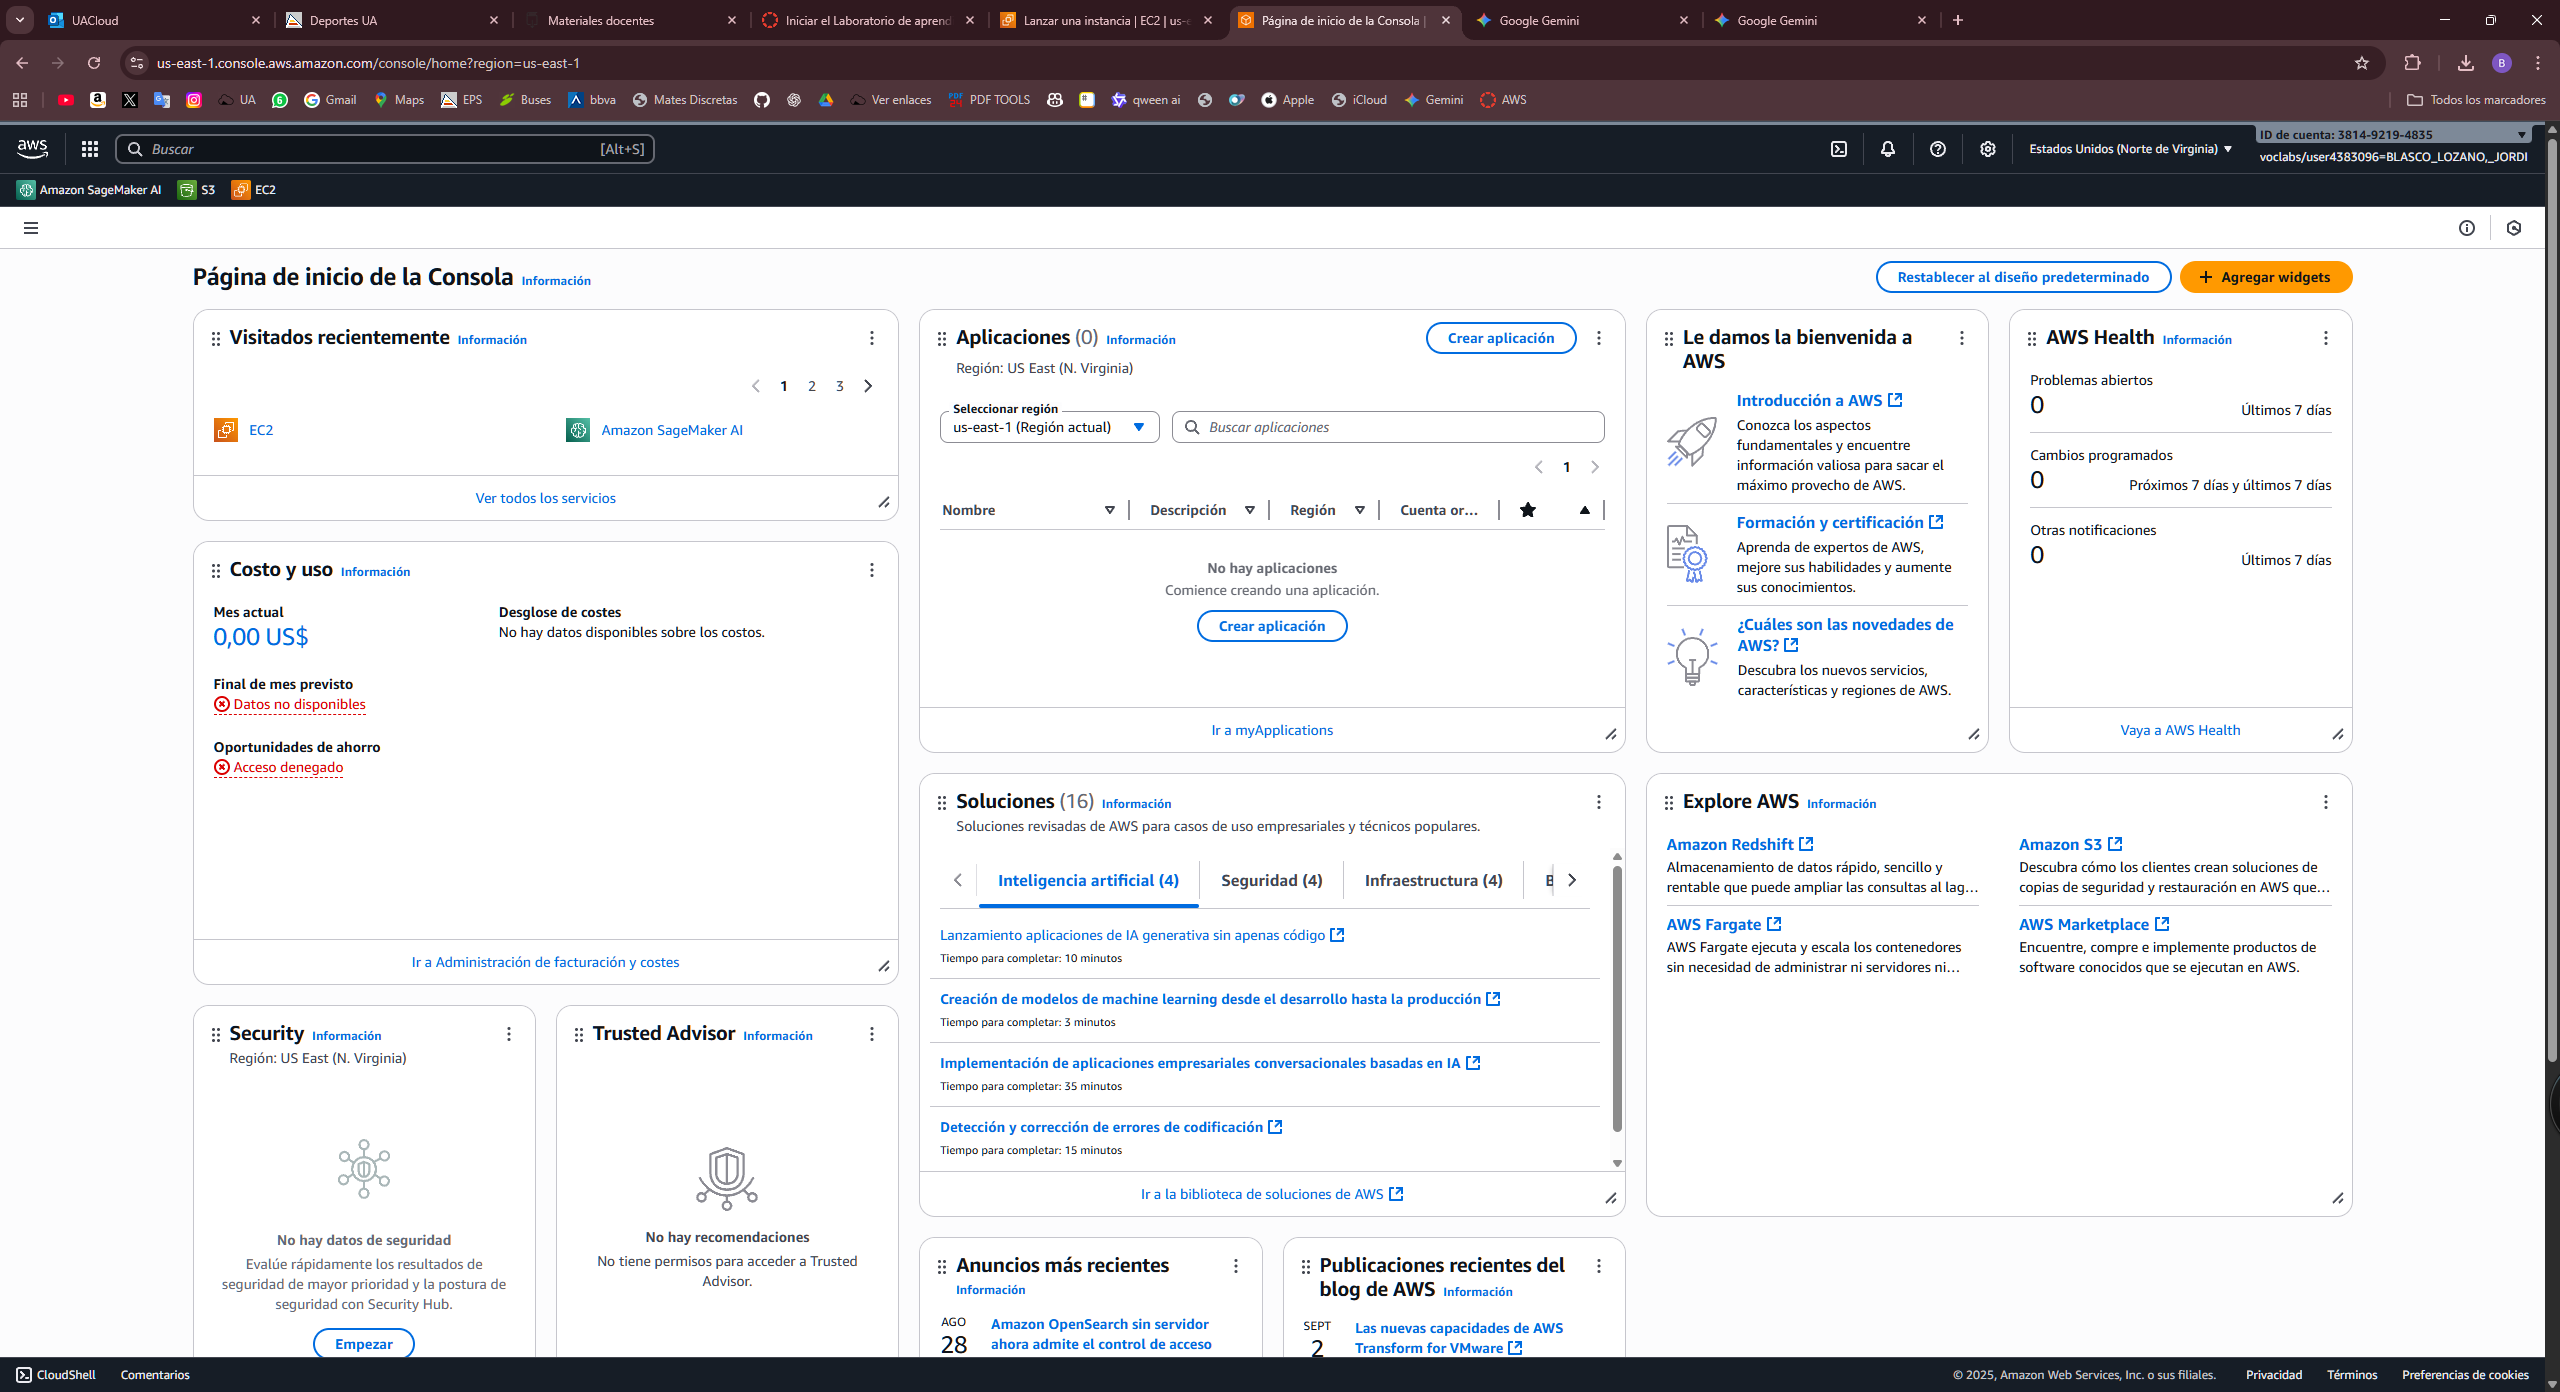
\includegraphics[width=0.95\textwidth]{tarea_1.png}
	\caption{Pantalla de inicio de sesión de AWS}
	\end{figure}

	\section{Exploración de Servicios}

	Una vez dentro de la consola, se puede acceder a una amplia variedad de servicios. Se accede a los servicios clicando en el botón de 9 puntos al lado del logo de AWS. Si buscamos los servicios que queramos podemos marcar los servicios favoritos para un acceso rápido dándole a la estrellita que aparece al lado del nombre del servicio.

	\begin{figure}[h!]
		\centering
		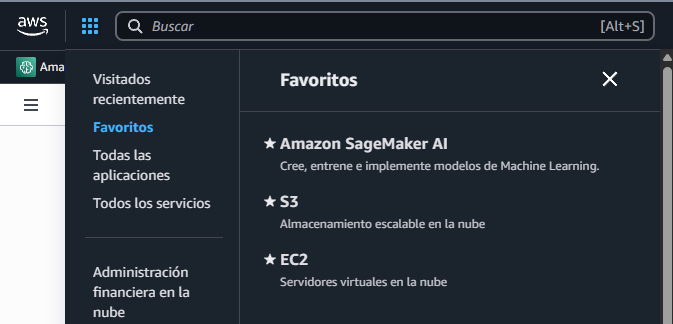
\includegraphics[width=0.95\textwidth]{tarea_2.png}
		\caption{Servicios favoritos}
		\end{figure}
	
	\newpage
	
	\section{Personalización de la Consola con Widgets}

	La consola permite personalizar la vista principal mediante widgets que muestran información relevante como el estado de los servicios, facturación y recursos recientes. La mayoría de los widgets están activados por defecto y si no lo están se pueden agregar dándole al botón de ``Agregar widgets'' qie se encuentra arriba a la derecha. He cambiado de posición los widgets de ``Visitados recientemente'', ``Costo y uso'' y ``AWS Health''.

	\begin{figure}[h!]
	\centering
	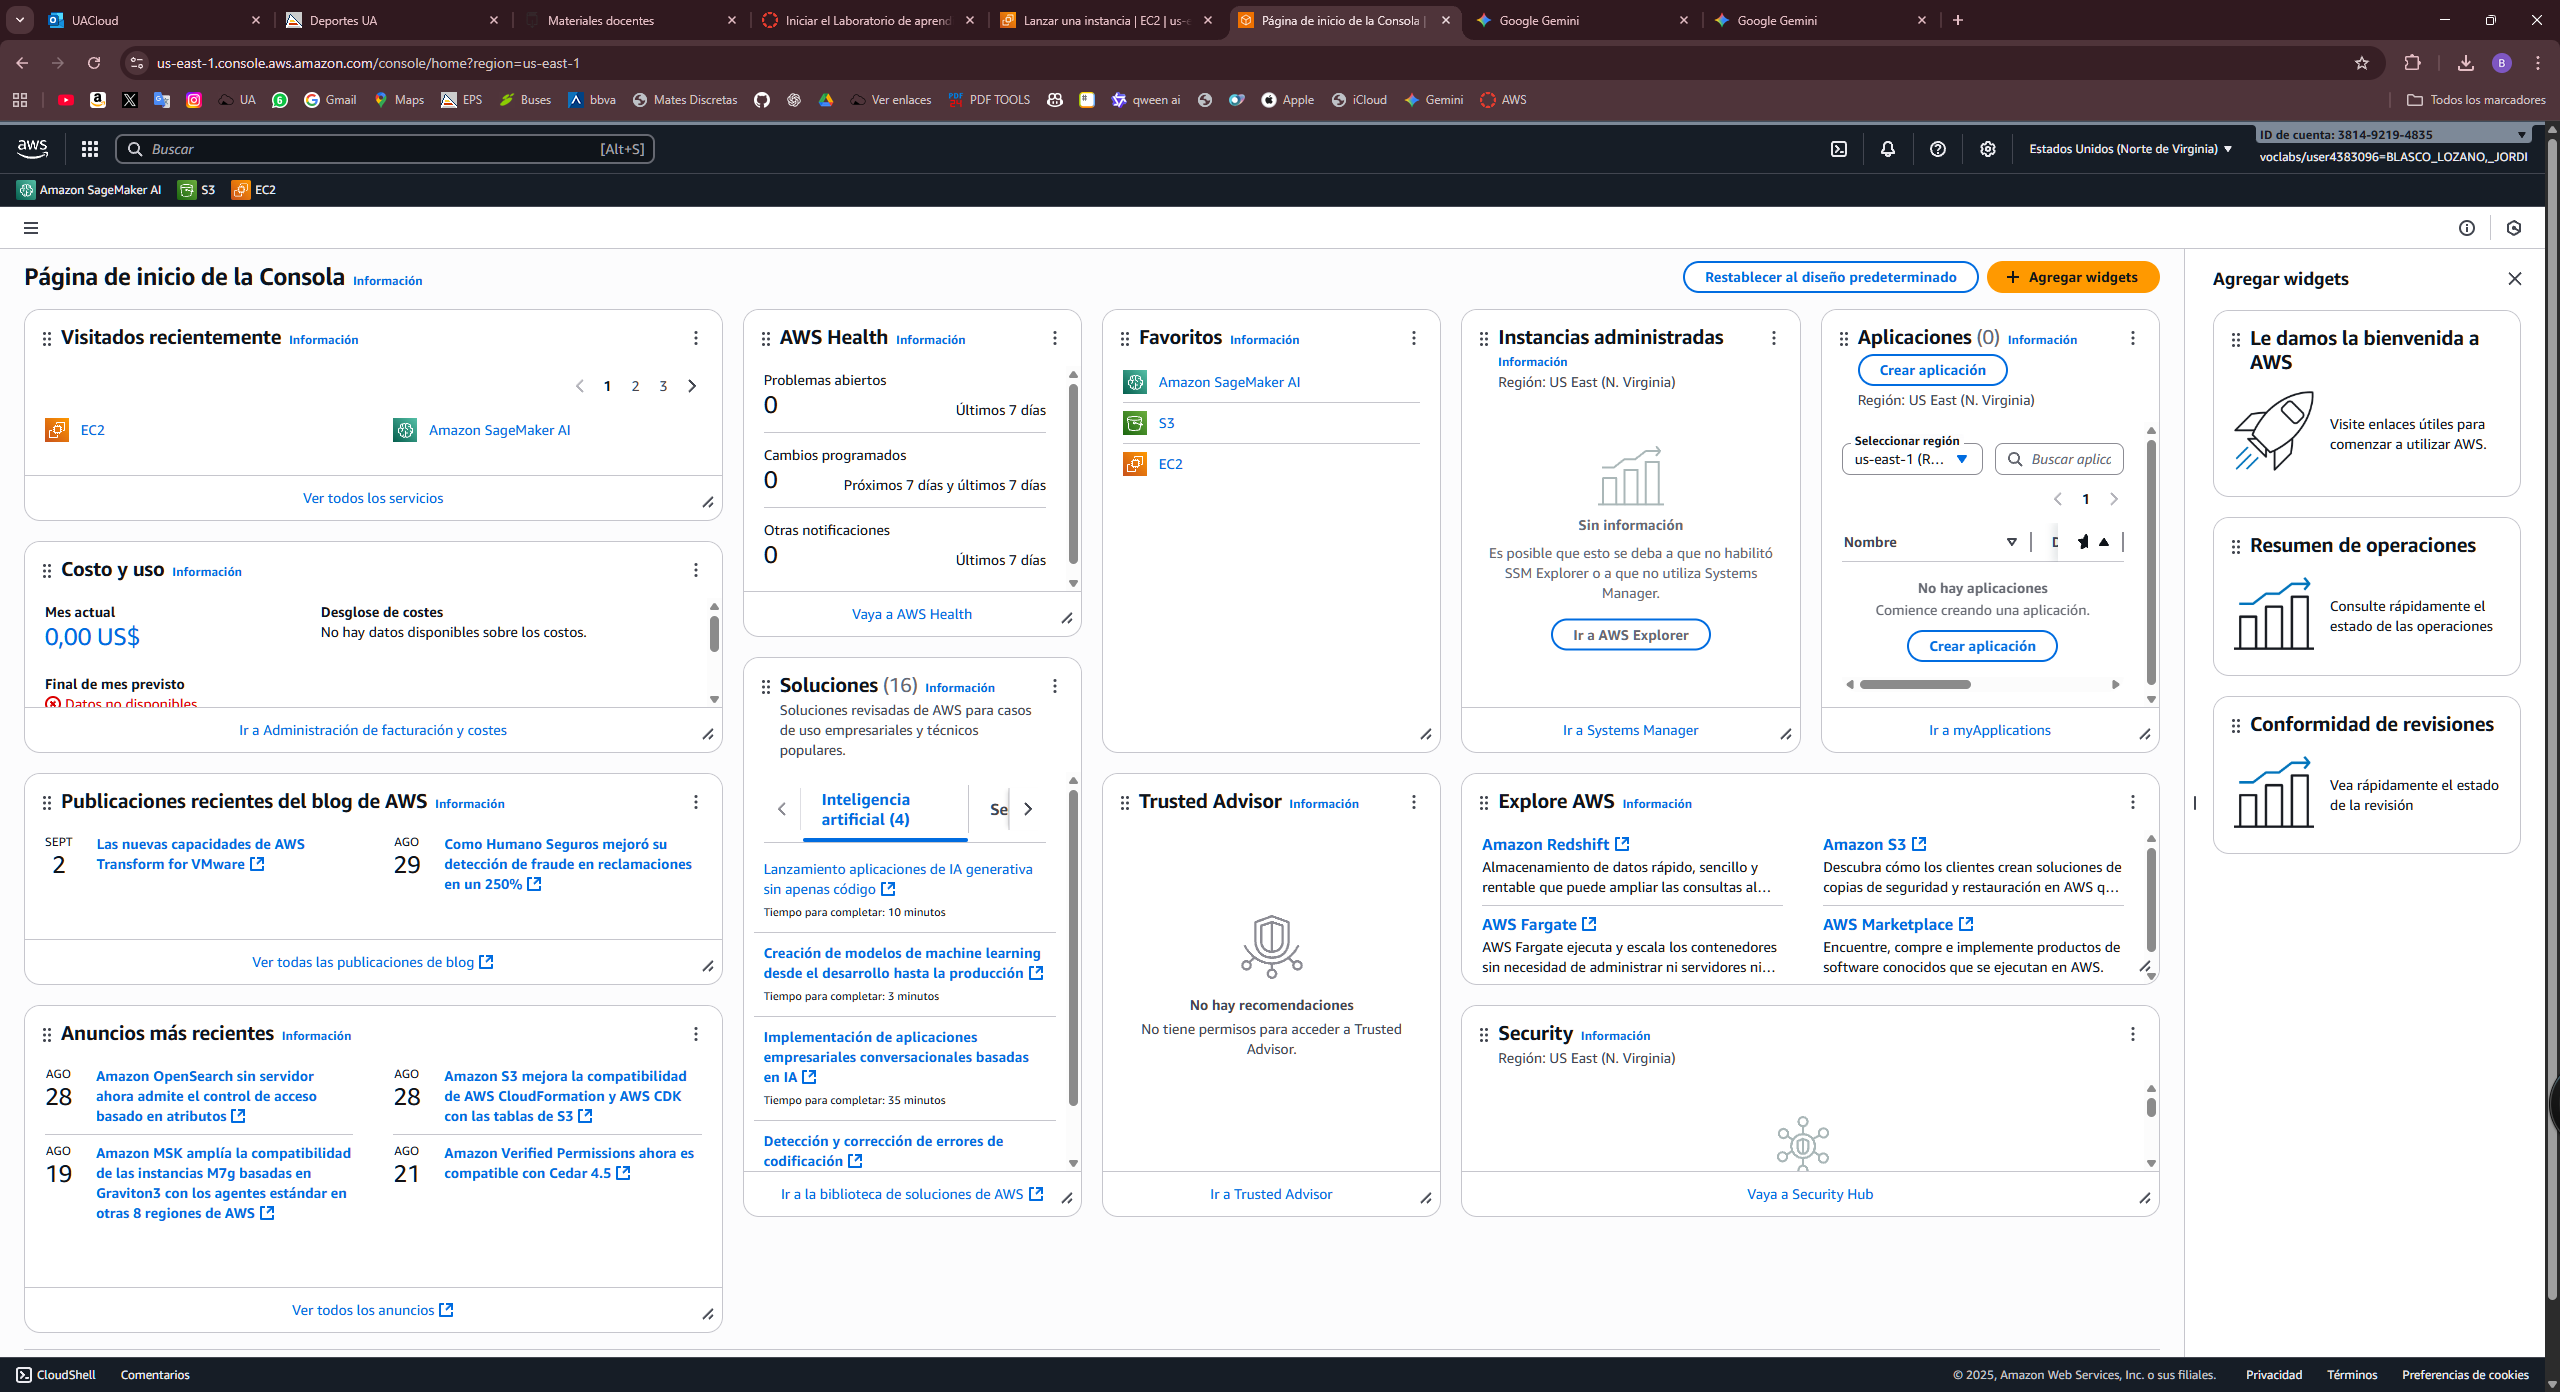
\includegraphics[width=0.95\textwidth]{tarea_3.png}
	\caption{Widgets de la pantalla de inicio}
	\end{figure}


	\section{Uso de MyApplications}

	MyApplications se utiliza para crear aplicaciones web que se ejecutan en AWS. Permite gestionar aplicaciones, configurar entornos y desplegar código de manera sencilla. Como no tenia ningún recurso he creado una aplicación vacía clicando en en crear aplicación y asgnandole un nombre.

	\begin{figure}[h!]
	\centering
	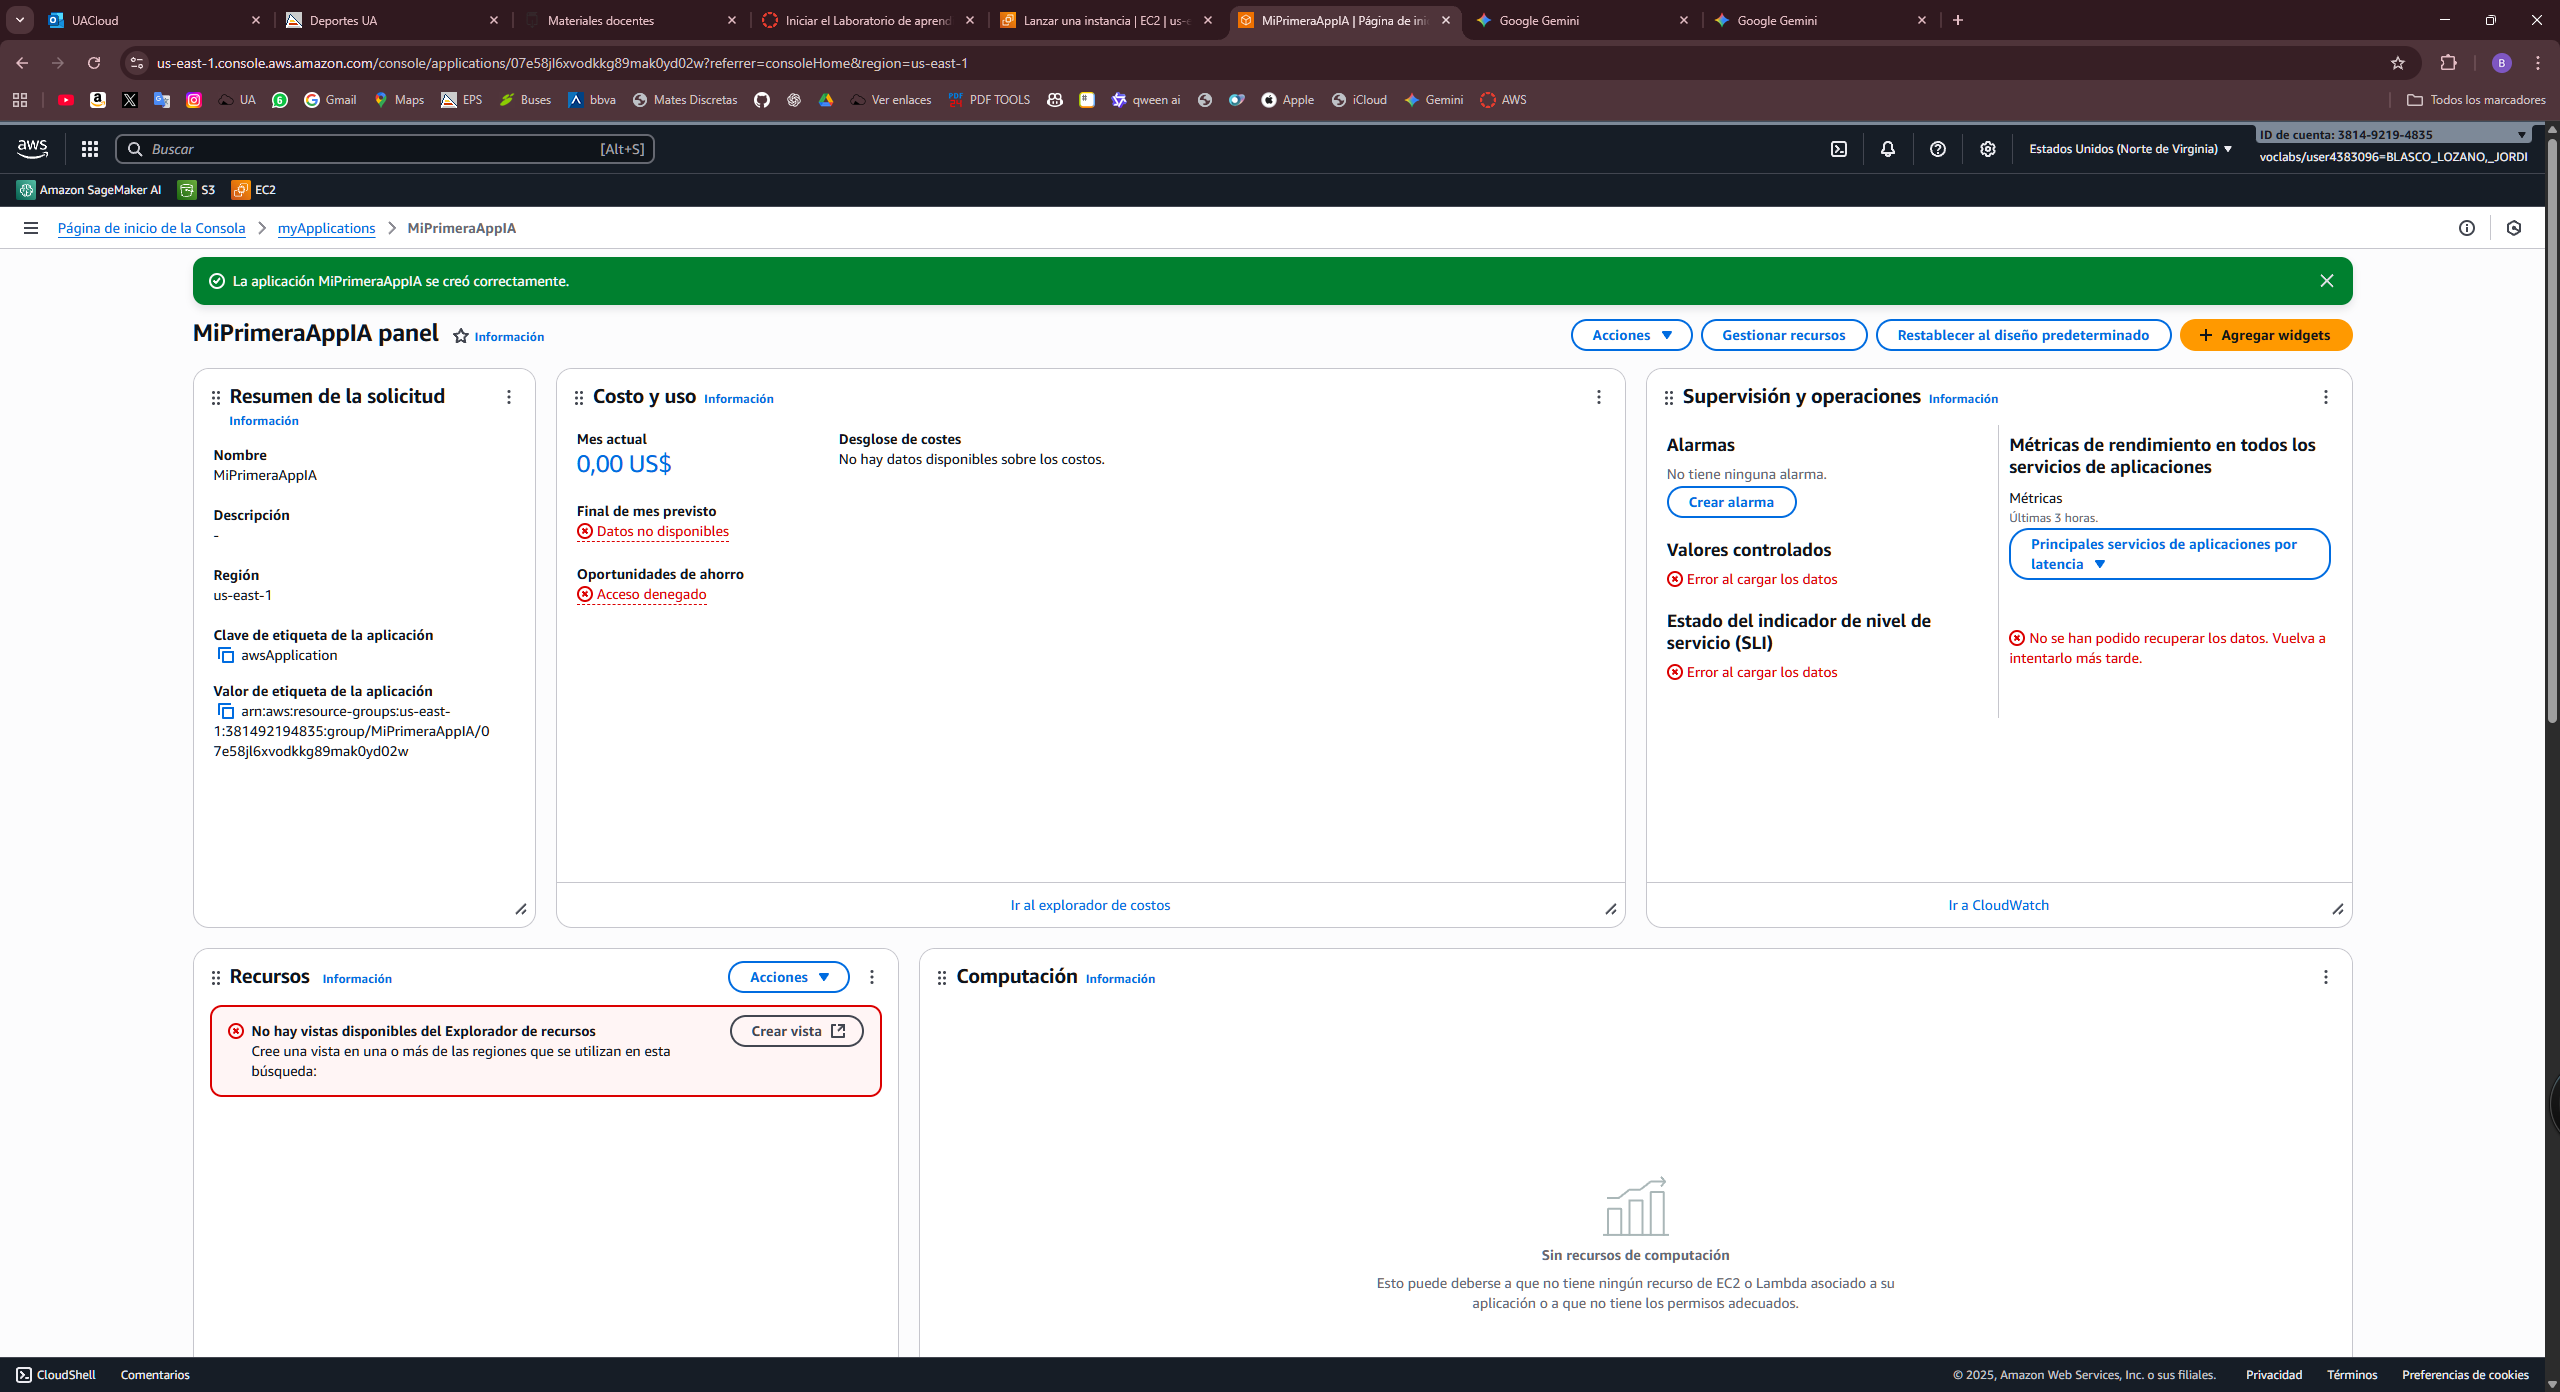
\includegraphics[width=0.95\textwidth]{tarea_4.png}
	\caption{Panel de MiPrimeraAppIA}
	\end{figure}

	\newpage

	\section{Búsqueda Eficiente}

	La consola de administración de AWS incluye una barra de búsqueda que permite encontrar rápidamente servicios y recursos. Si escribimos ``Cómo crear un bucket en S3'' se muestran servicios relacionados, publicaciones, documentación y artículos que son muy útiles para nuestra consulta.

	\begin{figure}[h!]
	\centering
	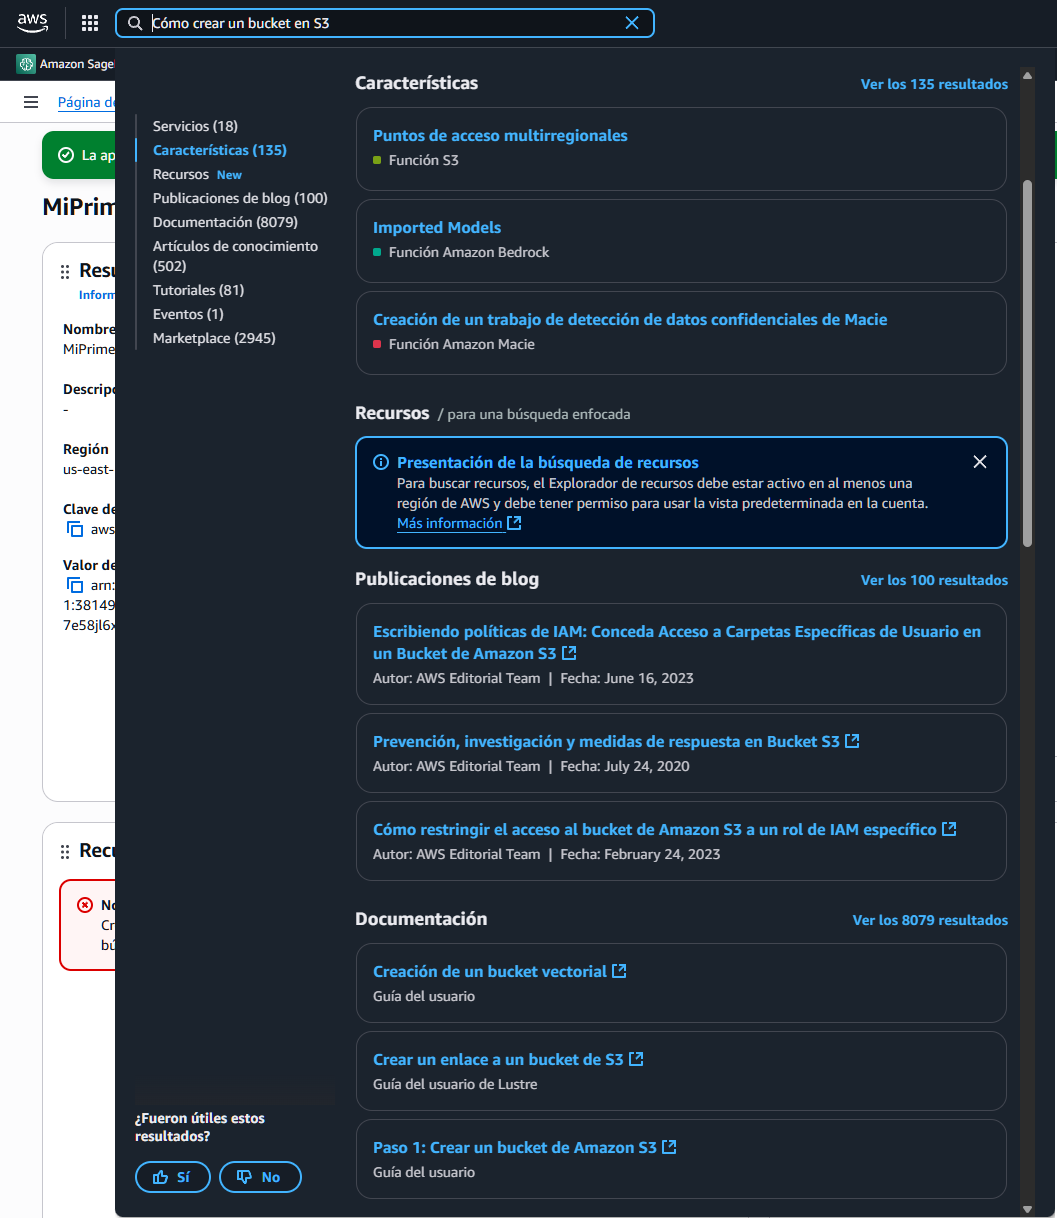
\includegraphics[width=0.95\textwidth]{tarea_5.png}
	\caption{Resultados de la búsqueda en la consola de AWS}
	\end{figure}

	\newpage

	\section{Interacción con Amazon Q}

	Amazon Q es un bot de inteligencia artificial al cual le podemos formular preguntas sobre AWS. Si le preguntamos ``¿Qué es Amazon SageMaker?'', nos proporciona una respuesta extensa y detallada sobre el servicio, en esta incluye características, ventajas, casos de uso y enlaces a documentación oficial o de la comunidad en la cual ha basado su respuesta. Tenemos un botón arriba a la derecha para poder llamarlo rápidamente.

	\begin{figure}[h!]
	\centering
	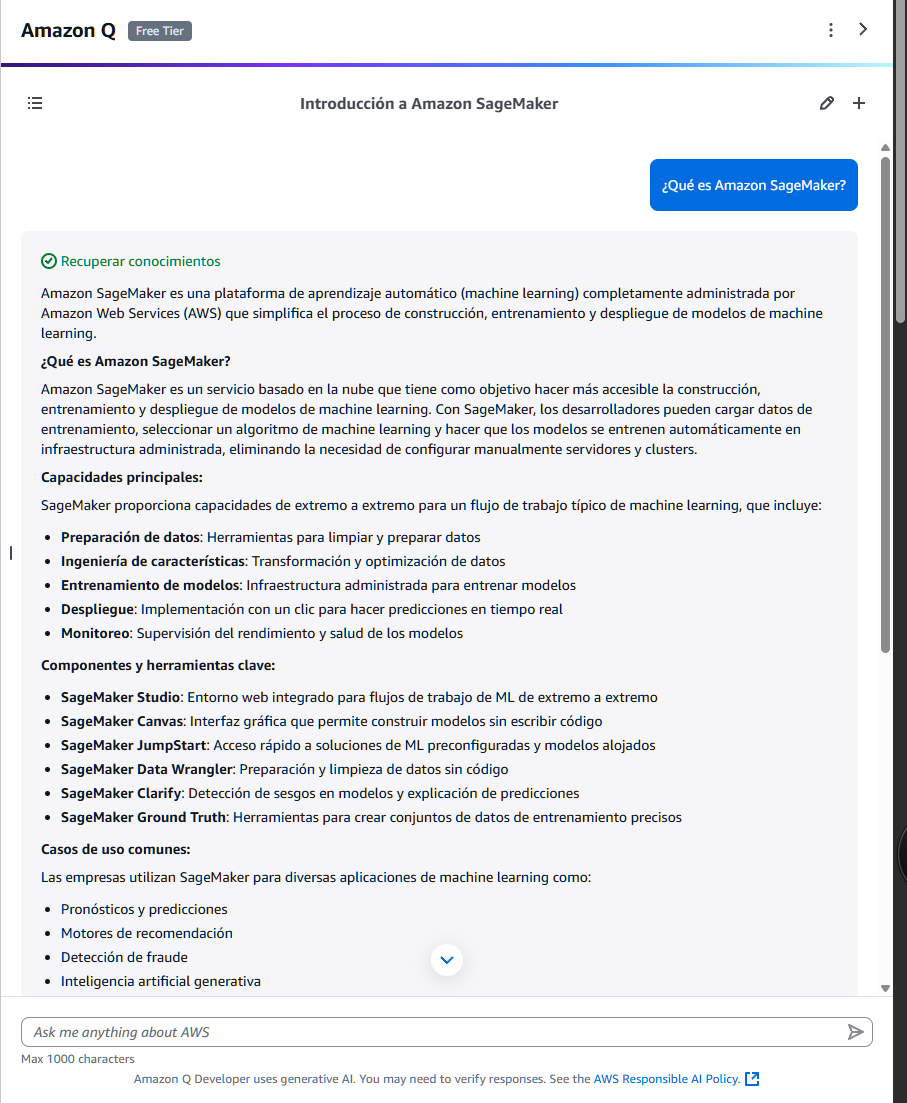
\includegraphics[width=0.95\textwidth]{tarea_6.png}
	\caption{Conversación con Amazon Q}
	\end{figure}

	\newpage

	\section{Gestión de Regiones}

	AWS tiene centros de datos en múltiples regiones alrededor del mundo. La región se puede cambiar desde el menú desplegable en la parte superior derecha de la consola. Por defecto, la región seleccionada es ``US East (N. Virginia)''. He cambiado la región a ``Europa (Irlanda) eu-west-1''.

	\begin{figure}[h!]
	\centering
	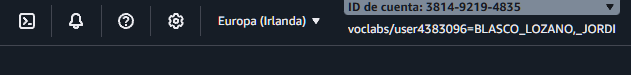
\includegraphics[width=0.95\textwidth]{tarea_7.png}
	\caption{Selección de región}
	\end{figure}

	\section{Exploración de la Consola de Costes y Facturación}

	Como AWS es un servicio de pago por uso, es fundamental entender cómo se facturan los servicios. La consola de Costes y Facturación proporciona herramientas para ver y analizar los costes, configurar alertas de presupuesto y revisar facturas detalladas. Se accede a ella directamente desde el widget del panel de consola de AWS.

	\begin{figure}[h!]
	\centering
	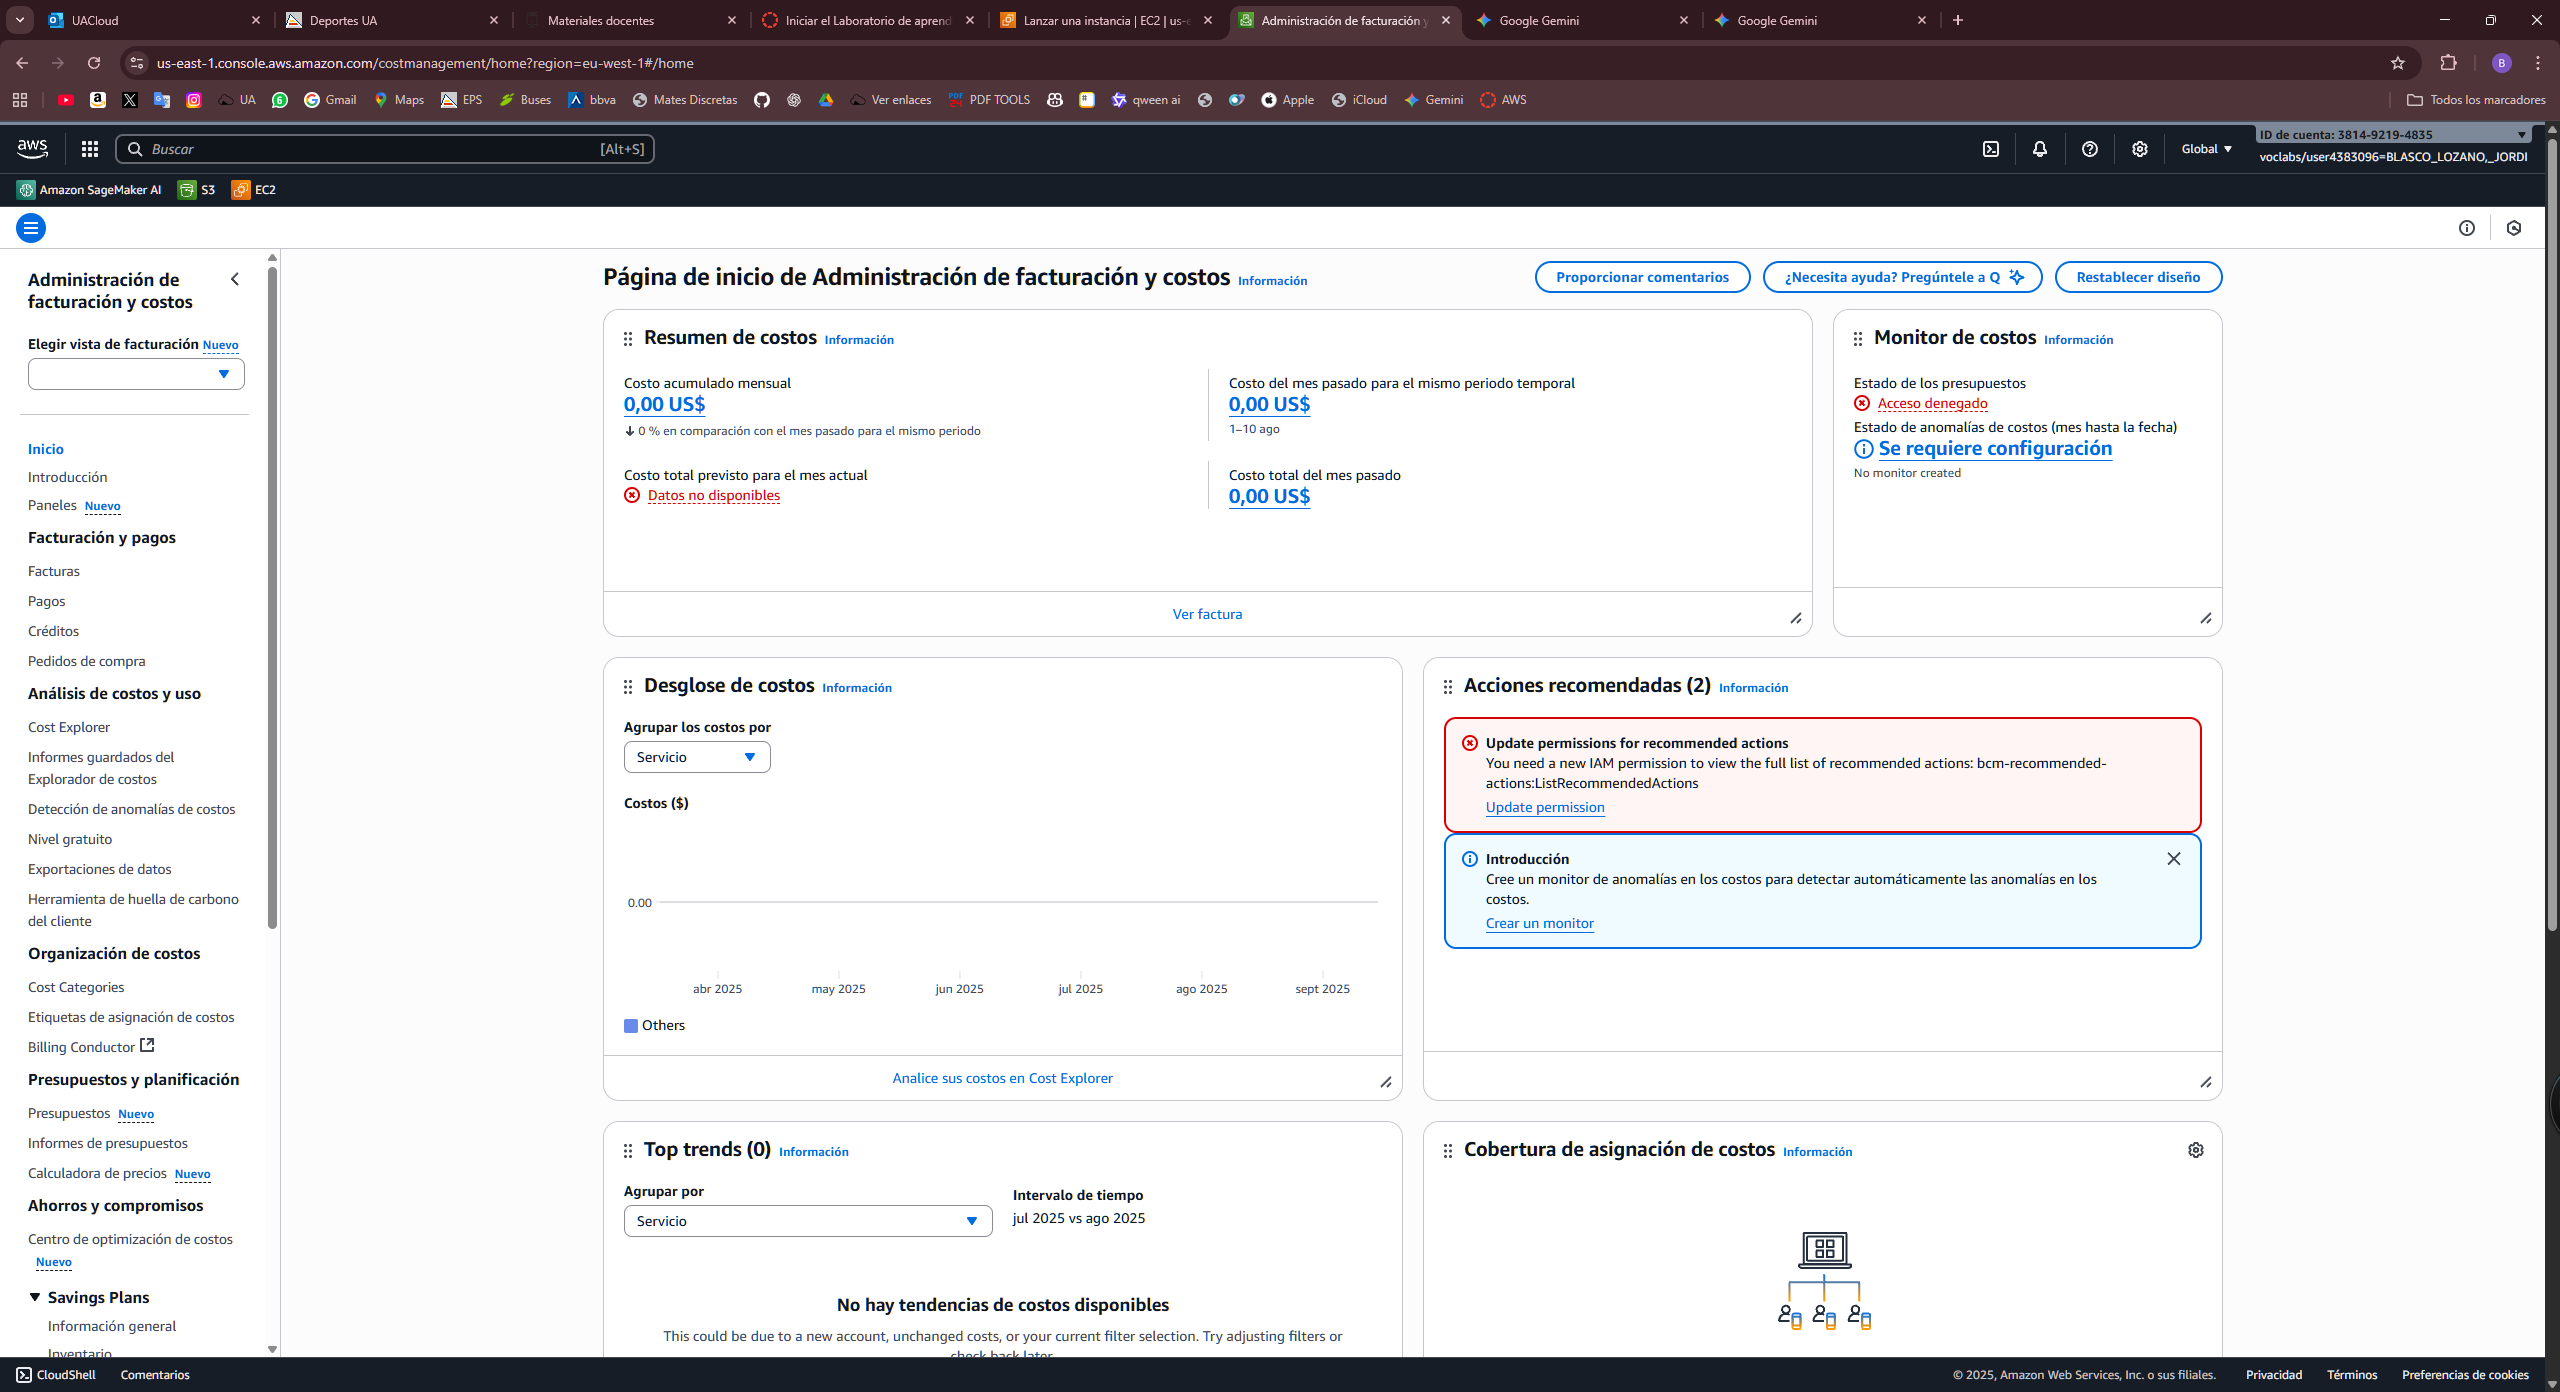
\includegraphics[width=0.95\textwidth]{tarea_8.png}
	\caption{Panel de Costes y Facturación}
	\end{figure}
	
	\clearpage

	\section{Tarea final}

	Para acabar haremos uso del servicio EC2, este servicio nos permite crear y gestionar instancias de servidores virtuales en la nube. Crearemos una instancia t3.micro con Amazon Linux, que son las configuraciones gratuitas y por defecto que ofrece Amazon. Una vez lanzada la instancia, nos conectaremos a ella mediante SSH utilizando un par de claves que he creado previamente. Para el comando utilizaré el comando proporcionado por AWS en la sección de conectarse a una instancia. Para hacer esto he tenido que buscar el servicio y darle a lanzar una instancia, después de esto se le debe de asignar un nombre y descargarte la clave ``.pem'' para poder acceder a ella mediante ssh, todos los valores de configuration se pueden dejar por defecto. Finalmente damos privilegios y accedemos por ssh desde nuestro terminal mediante los comandos que nos proporciona AWS en el apartado de ``conectarse a una instancia'' 


	\begin{figure}[H]
	\centering
	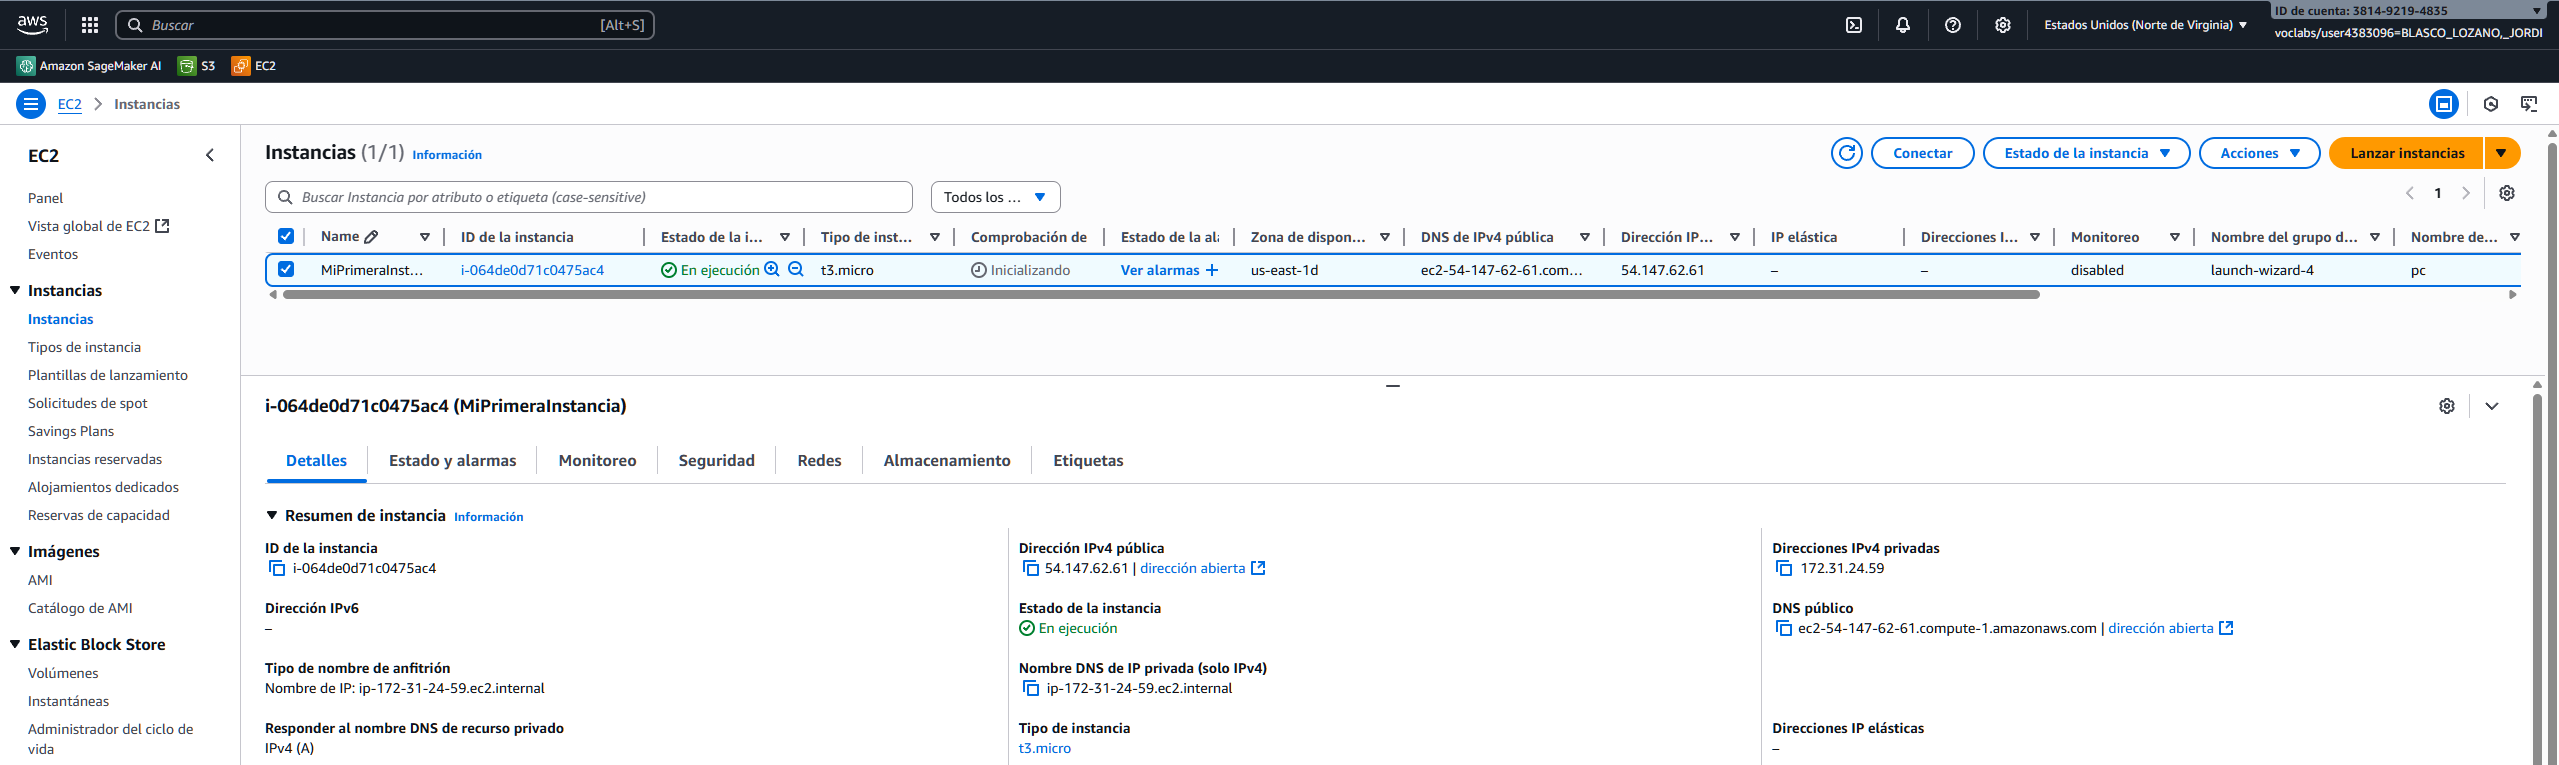
\includegraphics[width=0.95\textwidth]{tarea_final_1.png}
	\caption{Panel de instancias de EC2 con la instancia creada}
	\end{figure}



\begin{lstlisting}[style=consola, language=bash, caption={Salida de la terminal Windows Power Shell.}]
	PS C:\Users\jordi\Documents\UNI\IA\3erAnyo\1erCuatri\infraestructuras_y_servicios_cloud\practicas\practica_1> chmod 400 "pc.pem"
	PS  :\Users\jordi\Documents\UNI\IA\3erAnyo\1erCuatri\infraestructuras_y_servicios_cloud\practicas\practica_1> ssh -i "pc.pem" ec2-user@ec2-54-224-198-6.compute-1.amazonaws.com
	The authenticity of host 'ec2-54-224-198-6.compute-1.amazonaws.com (54.224.198.6)' can't be established.
	ED25519 key fingerprint is SHA256:70rYgLmu9wMm8ZWmCWcRWc7jPC/YBu6/XO29SwU94qk.
	This key is not known by any other names.
	Are you sure you want to continue connecting (yes/no/[fingerprint])? yes
	Warning: Permanently added 'ec2-54-224-198-6.compute-1.amazonaws.com' (ED25519) to the list of known hosts.
	,     #_
	~\_  ####_        Amazon Linux 2023
	~~  \_#####\
	~~   \###|
	~~       \#/ ___   https://aws.amazon.com/linux/amazon-linux-2023
	~~       V~' '->
		~~~         /
		~~._.   _/
			_/ _/
		_/m/'
	[ec2-user@ip-172-31-27-182 ~]$ ls
	[ec2-user@ip-172-31-27-182 ~]$ mkdir hola
	[ec2-user@ip-172-31-27-182 ~]$ ls
	hola
	[ec2-user@ip-172-31-27-182 ~]$

\end{lstlisting}

\end{document}
